\clearpage
\myparagraph{\RU{Первый пример с \olly: a=1,2 и и=3,4}\EN{First \olly example: a=1.2 and b=3.4}}
\index{\olly}

\RU{Обе}\EN{Both} \FLD \RU{отработали}\EN{are executed}:

\begin{figure}[H]
\centering
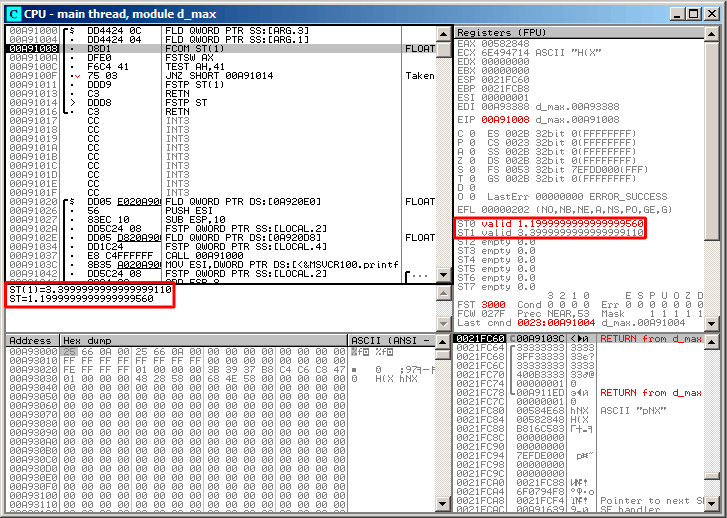
\includegraphics[scale=\FigScale]{patterns/12_FPU/3_comparison/x86/MSVC_Ox/olly1_1.png}
\caption{\olly: \RU{обе \FLD исполнились}\EN{both \FLD are executed}}
\label{fig:FPU_comparison_Ox_case1_olly1}
\end{figure}

\RU{Сейчас будет исполняться }\FCOM\EN{ being executed}: 
\olly \RU{показывает содержимое}\EN{shows the contents of} \ST{0} \AndENRU \ST{1} \RU{для удобства}%
\EN{for convenience}.

\clearpage
\FCOM \RU{сработала}\EN{is done}:

\begin{figure}[H]
\centering
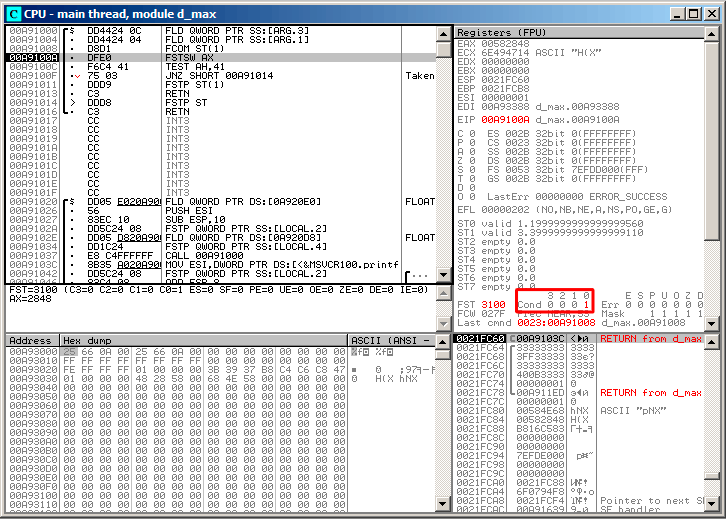
\includegraphics[scale=\FigScale]{patterns/12_FPU/3_comparison/x86/MSVC_Ox/olly1_2.png}
\caption{\olly: \FCOM \RU{исполнилась}\EN{is done}}
\label{fig:FPU_comparison_Ox_case1_olly2}
\end{figure}

\Czero \RU{установлен, остальные флаги сброшены}\EN{is set, all other condition flags are cleared}.

\clearpage
\FNSTSW \RU{сработала}\EN{is done}, \GTT{AX}=0x3100:

\begin{figure}[H]
\centering
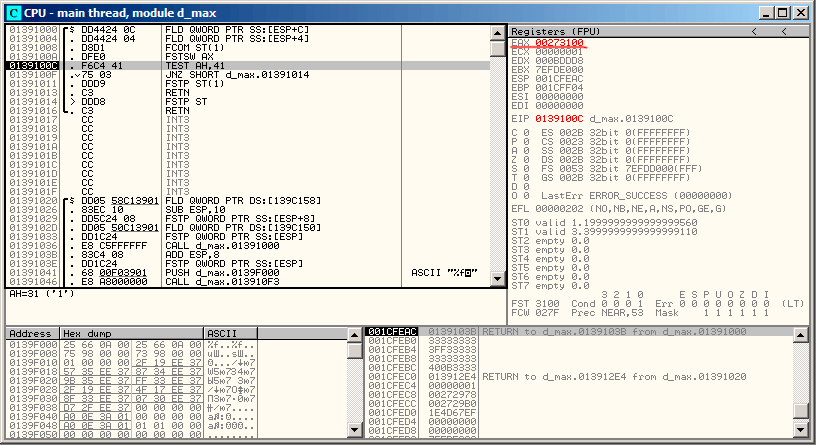
\includegraphics[scale=\FigScale]{patterns/12_FPU/3_comparison/x86/MSVC_Ox/olly1_3.png}
\caption{\olly: \FNSTSW \RU{исполнилась}\EN{is executed}}
\label{fig:FPU_comparison_Ox_case1_olly3}
\end{figure}

\clearpage
\TEST \RU{сработала}\EN{is executed}:

\begin{figure}[H]
\centering
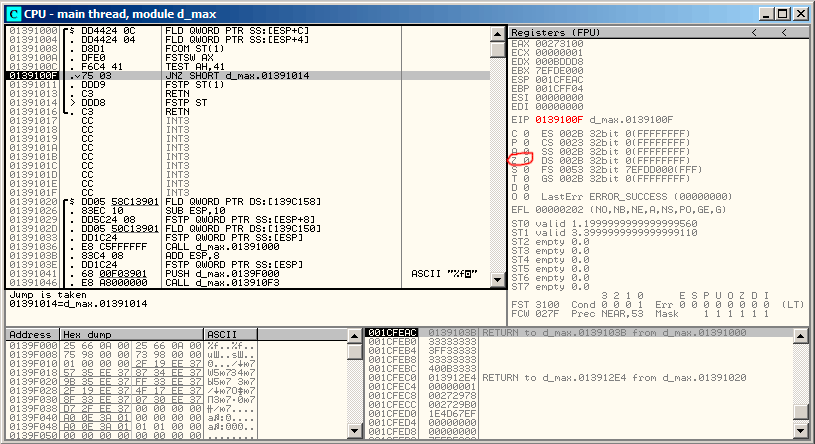
\includegraphics[scale=\FigScale]{patterns/12_FPU/3_comparison/x86/MSVC_Ox/olly1_4.png}
\caption{\olly: \TEST \RU{исполнилась}\EN{is executed}}
\label{fig:FPU_comparison_Ox_case1_olly4}
\end{figure}

ZF=0, \RU{переход сейчас произойдет}\EN{conditional jump is about to trigger now}.

\clearpage
\INS{FSTP ST} (\OrENRU \FSTP \ST{0}) \RU{сработала}\EN{was executed}~---%
\RU{ 1,2 было вытолкнуто из стека, и на вершине осталось 3,4}%
\EN{1.2 was popped from the stack, and 3.4 was left on top}:

\begin{figure}[H]
\centering
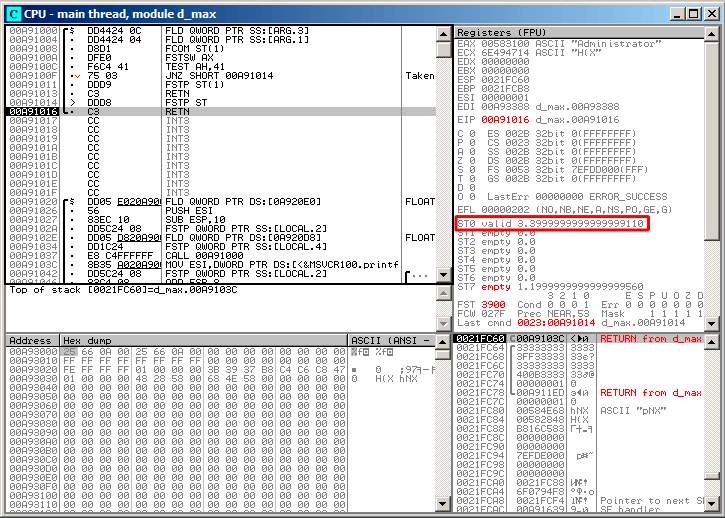
\includegraphics[scale=\FigScale]{patterns/12_FPU/3_comparison/x86/MSVC_Ox/olly1_5.png}
\caption{\olly: \FSTP \RU{исполнилась}\EN{is executed}}
\label{fig:FPU_comparison_Ox_case1_olly5}
\end{figure}

\RU{Видно, что инструкция}\EN{We see that the} \INS{FSTP ST} 
\RU{работает просто как выталкивание одного значения из FPU-стека.}
\EN{instruction works just like popping one value from the FPU stack.}

\clearpage
\myparagraph{\RU{Второй пример с \olly: a=5,6 и b=-4}\EN{Second \olly example: a=5.6 and b=-4}}

\RU{Обе}\EN{Both} \FLD \RU{отработали}\EN{are executed}:

\begin{figure}[H]
\centering
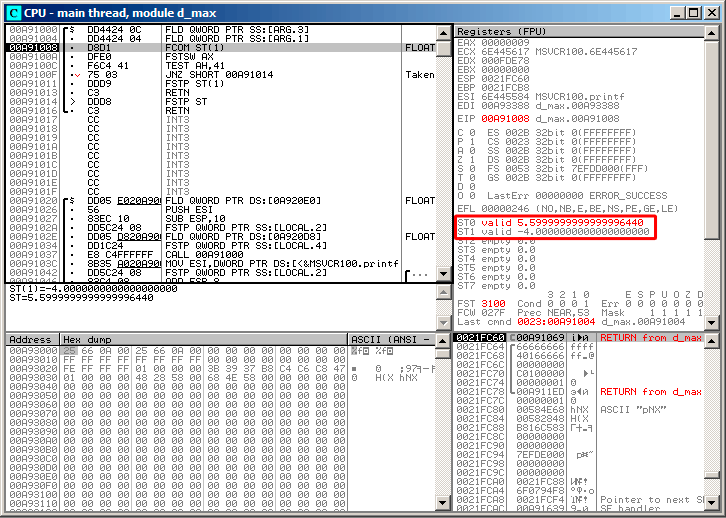
\includegraphics[scale=\FigScale]{patterns/12_FPU/3_comparison/x86/MSVC_Ox/olly2_1.png}
\caption{\olly: \RU{обе \FLD исполнились}\EN{both \FLD are executed}}
\label{fig:FPU_comparison_Ox_case2_olly1}
\end{figure}

\RU{Сейчас будет исполняться \FCOM.}
\EN{\FCOM is about to execute.}

\clearpage
\FCOM \RU{сработала}\EN{is done}:

\begin{figure}[H]
\centering
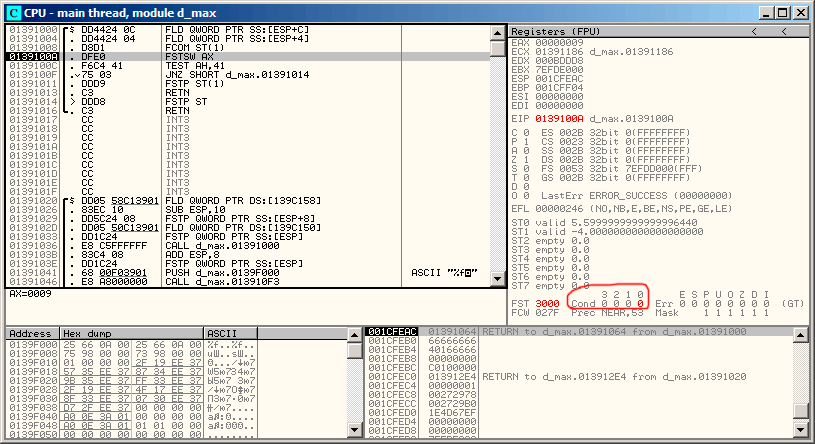
\includegraphics[scale=\FigScale]{patterns/12_FPU/3_comparison/x86/MSVC_Ox/olly2_2.png}
\caption{\olly: \FCOM \RU{исполнилась}\EN{is finished}}
\label{fig:FPU_comparison_Ox_case2_olly2}
\end{figure}

\RU{Все condition-флаги сброшены}\EN{All conditional flags are cleared}.

\clearpage
\FNSTSW \RU{сработала}\EN{done}, \GTT{AX}=0x3000:

\begin{figure}[H]
\centering
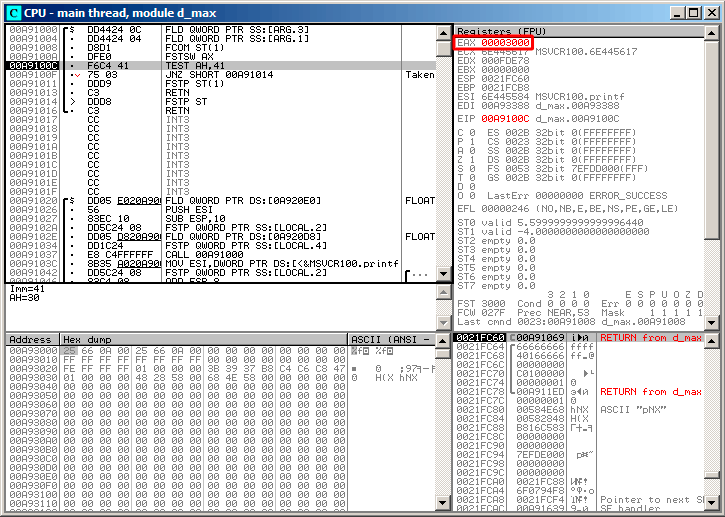
\includegraphics[scale=\FigScale]{patterns/12_FPU/3_comparison/x86/MSVC_Ox/olly2_3.png}
\caption{\olly: \FNSTSW \RU{исполнилась}\EN{was executed}}
\label{fig:FPU_comparison_Ox_case2_olly3}
\end{figure}

\clearpage
\TEST \RU{сработала}\EN{is done}:

\begin{figure}[H]
\centering
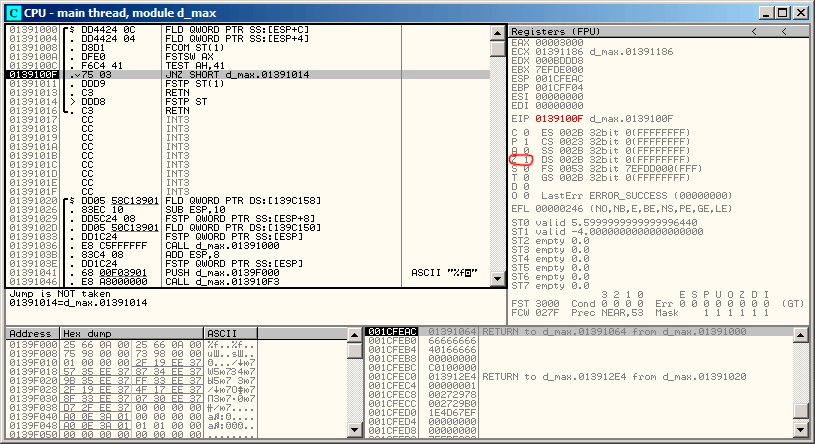
\includegraphics[scale=\FigScale]{patterns/12_FPU/3_comparison/x86/MSVC_Ox/olly2_4.png}
\caption{\olly: \TEST \RU{исполнилась}\EN{was executed}}
\label{fig:FPU_comparison_Ox_case2_olly4}
\end{figure}

ZF=1, \RU{переход сейчас не произойдет}\EN{jump will not happen now}.

\clearpage
\FSTP \ST{1} \RU{сработала: на вершине FPU-стека осталось значение 5,6}\EN{was executed: a value
of 5.6 is now at the top of the FPU stack}.

\begin{figure}[H]
\centering
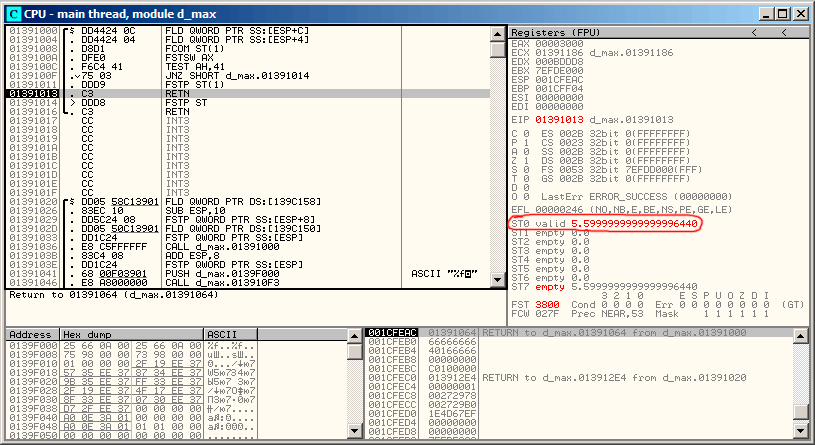
\includegraphics[scale=\FigScale]{patterns/12_FPU/3_comparison/x86/MSVC_Ox/olly2_5.png}
\caption{\olly: \FSTP \RU{исполнилась}\EN{was executed}}
\label{fig:FPU_comparison_Ox_case2_olly5}
\end{figure}

\RU{Видно, что инструкция}\EN{We now see that the} \FSTP \ST{1} 
\RU{работает так: оставляет значение на вершине стека, но обнуляет регистр \ST{1}.}
\EN{instruction works as follows: it leaves what was at the top of the stack, but clears \ST{1}.}
